\documentclass[tikz,border=6pt]{standalone}
\usepackage{tikz}
\begin{document}
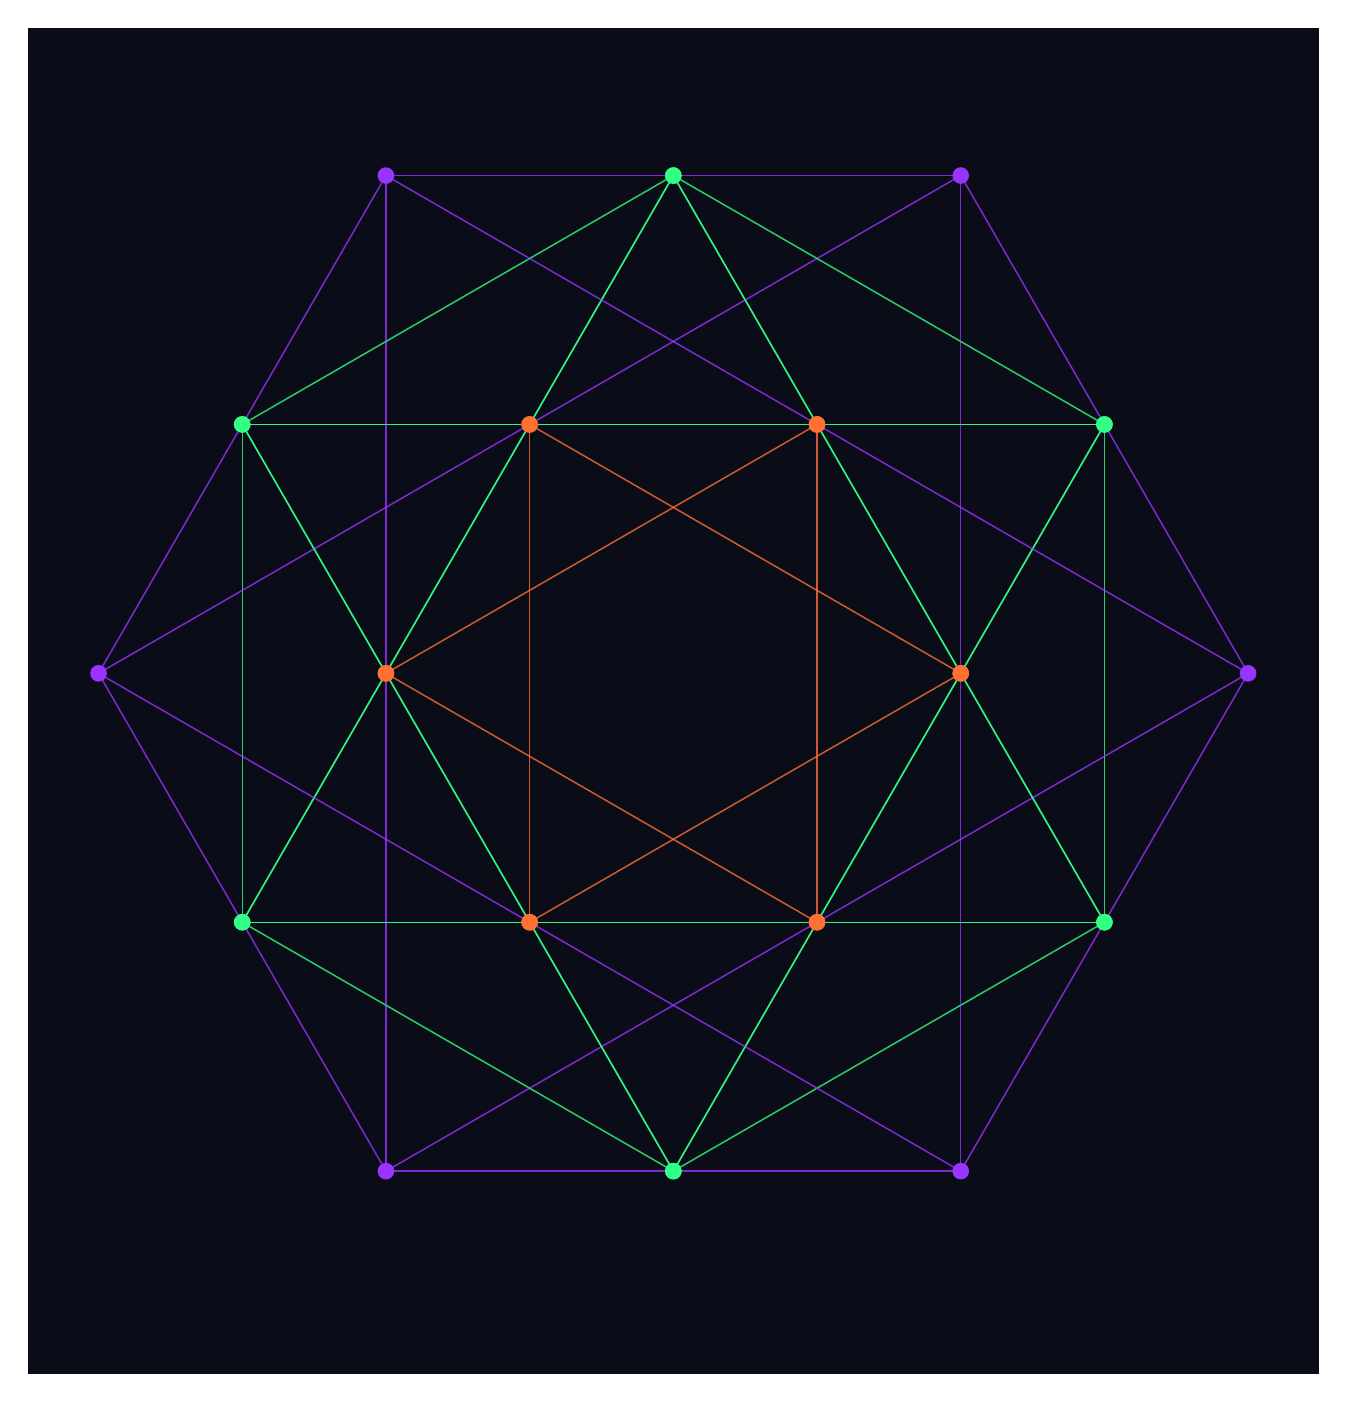
\begin{tikzpicture}
\definecolor{ring0}{rgb}{1.000,0.440,0.200}
\definecolor{ring1}{rgb}{0.200,1.000,0.520}
\definecolor{ring2}{rgb}{0.600,0.200,1.000}
\definecolor{bg}{rgb}{0.04,0.05,0.09}
\fill[bg] (-8.2,-8.9) rectangle (8.2,8.2);
\draw[ring1,line width=0.5pt,opacity=0.55] (-1.825,3.161)--(-0.000,6.322);
\draw[ring2,line width=0.5pt,opacity=0.55] (-1.825,3.161)--(3.650,6.322);
\draw[ring1,line width=0.5pt,opacity=0.55] (-1.825,3.161)--(5.475,3.161);
\draw[ring0,line width=0.5pt,opacity=0.55] (-1.825,3.161)--(3.650,0.000);
\draw[ring0,line width=0.5pt,opacity=0.55] (-1.825,3.161)--(-1.825,-3.161);
\draw[ring1,line width=0.5pt,opacity=0.55] (-1.825,3.161)--(-5.475,-3.161);
\draw[ring2,line width=0.5pt,opacity=0.55] (-1.825,3.161)--(-7.300,-0.000);
\draw[ring1,line width=0.5pt,opacity=0.55] (-1.825,3.161)--(-5.475,3.161);
\draw[ring2,line width=0.5pt,opacity=0.55] (-0.000,6.322)--(3.650,6.322);
\draw[ring1,line width=0.5pt,opacity=0.55] (-0.000,6.322)--(5.475,3.161);
\draw[ring1,line width=0.5pt,opacity=0.55] (-0.000,6.322)--(3.650,0.000);
\draw[ring1,line width=0.5pt,opacity=0.55] (-0.000,6.322)--(1.825,3.161);
\draw[ring1,line width=0.5pt,opacity=0.55] (-0.000,6.322)--(-3.650,-0.000);
\draw[ring1,line width=0.5pt,opacity=0.55] (-0.000,6.322)--(-5.475,3.161);
\draw[ring2,line width=0.5pt,opacity=0.55] (-0.000,6.322)--(-3.650,6.322);
\draw[ring2,line width=0.5pt,opacity=0.55] (3.650,6.322)--(5.475,3.161);
\draw[ring2,line width=0.5pt,opacity=0.55] (3.650,6.322)--(3.650,0.000);
\draw[ring2,line width=0.5pt,opacity=0.55] (3.650,6.322)--(5.475,3.161);
\draw[ring2,line width=0.5pt,opacity=0.55] (3.650,6.322)--(3.650,0.000);
\draw[ring2,line width=0.5pt,opacity=0.55] (3.650,6.322)--(-1.825,3.161);
\draw[ring2,line width=0.5pt,opacity=0.55] (3.650,6.322)--(-0.000,6.322);
\draw[ring1,line width=0.5pt,opacity=0.55] (5.475,3.161)--(3.650,0.000);
\draw[ring2,line width=0.5pt,opacity=0.55] (5.475,3.161)--(7.300,0.000);
\draw[ring1,line width=0.5pt,opacity=0.55] (5.475,3.161)--(5.475,-3.161);
\draw[ring1,line width=0.5pt,opacity=0.55] (5.475,3.161)--(1.825,-3.161);
\draw[ring1,line width=0.5pt,opacity=0.55] (5.475,3.161)--(1.825,3.161);
\draw[ring1,line width=0.5pt,opacity=0.55] (3.650,0.000)--(5.475,-3.161);
\draw[ring2,line width=0.5pt,opacity=0.55] (3.650,0.000)--(3.650,-6.322);
\draw[ring1,line width=0.5pt,opacity=0.55] (3.650,0.000)--(0.000,-6.322);
\draw[ring0,line width=0.5pt,opacity=0.55] (3.650,0.000)--(-1.825,-3.161);
\draw[ring0,line width=0.5pt,opacity=0.55] (1.825,-3.161)--(1.825,3.161);
\draw[ring1,line width=0.5pt,opacity=0.55] (1.825,-3.161)--(5.475,3.161);
\draw[ring2,line width=0.5pt,opacity=0.55] (1.825,-3.161)--(7.300,0.000);
\draw[ring1,line width=0.5pt,opacity=0.55] (1.825,-3.161)--(5.475,-3.161);
\draw[ring1,line width=0.5pt,opacity=0.55] (1.825,-3.161)--(0.000,-6.322);
\draw[ring2,line width=0.5pt,opacity=0.55] (1.825,-3.161)--(-3.650,-6.322);
\draw[ring1,line width=0.5pt,opacity=0.55] (1.825,-3.161)--(-5.475,-3.161);
\draw[ring0,line width=0.5pt,opacity=0.55] (1.825,-3.161)--(-3.650,-0.000);
\draw[ring1,line width=0.5pt,opacity=0.55] (1.825,3.161)--(5.475,3.161);
\draw[ring2,line width=0.5pt,opacity=0.55] (1.825,3.161)--(7.300,0.000);
\draw[ring1,line width=0.5pt,opacity=0.55] (1.825,3.161)--(5.475,-3.161);
\draw[ring0,line width=0.5pt,opacity=0.55] (1.825,3.161)--(-3.650,-0.000);
\draw[ring1,line width=0.5pt,opacity=0.55] (1.825,3.161)--(-5.475,3.161);
\draw[ring2,line width=0.5pt,opacity=0.55] (1.825,3.161)--(-3.650,6.322);
\draw[ring2,line width=0.5pt,opacity=0.55] (5.475,3.161)--(7.300,0.000);
\draw[ring1,line width=0.5pt,opacity=0.55] (5.475,3.161)--(5.475,-3.161);
\draw[ring1,line width=0.5pt,opacity=0.55] (5.475,3.161)--(3.650,0.000);
\draw[ring1,line width=0.5pt,opacity=0.55] (5.475,3.161)--(-1.825,3.161);
\draw[ring1,line width=0.5pt,opacity=0.55] (5.475,3.161)--(-0.000,6.322);
\draw[ring2,line width=0.5pt,opacity=0.55] (7.300,0.000)--(5.475,-3.161);
\draw[ring2,line width=0.5pt,opacity=0.55] (7.300,0.000)--(5.475,-3.161);
\draw[ring2,line width=0.5pt,opacity=0.55] (7.300,0.000)--(1.825,-3.161);
\draw[ring2,line width=0.5pt,opacity=0.55] (7.300,0.000)--(1.825,3.161);
\draw[ring2,line width=0.5pt,opacity=0.55] (5.475,-3.161)--(3.650,-6.322);
\draw[ring1,line width=0.5pt,opacity=0.55] (5.475,-3.161)--(0.000,-6.322);
\draw[ring1,line width=0.5pt,opacity=0.55] (5.475,-3.161)--(-1.825,-3.161);
\draw[ring1,line width=0.5pt,opacity=0.55] (0.000,-6.322)--(-1.825,-3.161);
\draw[ring1,line width=0.5pt,opacity=0.55] (0.000,-6.322)--(3.650,0.000);
\draw[ring1,line width=0.5pt,opacity=0.55] (0.000,-6.322)--(5.475,-3.161);
\draw[ring2,line width=0.5pt,opacity=0.55] (0.000,-6.322)--(3.650,-6.322);
\draw[ring2,line width=0.5pt,opacity=0.55] (0.000,-6.322)--(-3.650,-6.322);
\draw[ring1,line width=0.5pt,opacity=0.55] (0.000,-6.322)--(-5.475,-3.161);
\draw[ring1,line width=0.5pt,opacity=0.55] (0.000,-6.322)--(-3.650,-0.000);
\draw[ring0,line width=0.5pt,opacity=0.55] (-1.825,-3.161)--(3.650,0.000);
\draw[ring1,line width=0.5pt,opacity=0.55] (-1.825,-3.161)--(5.475,-3.161);
\draw[ring2,line width=0.5pt,opacity=0.55] (-1.825,-3.161)--(3.650,-6.322);
\draw[ring1,line width=0.5pt,opacity=0.55] (-1.825,-3.161)--(-5.475,-3.161);
\draw[ring2,line width=0.5pt,opacity=0.55] (-1.825,-3.161)--(-7.300,-0.000);
\draw[ring1,line width=0.5pt,opacity=0.55] (-1.825,-3.161)--(-5.475,3.161);
\draw[ring1,line width=0.5pt,opacity=0.55] (3.650,0.000)--(5.475,-3.161);
\draw[ring2,line width=0.5pt,opacity=0.55] (3.650,0.000)--(3.650,-6.322);
\draw[ring0,line width=0.5pt,opacity=0.55] (3.650,0.000)--(-1.825,3.161);
\draw[ring1,line width=0.5pt,opacity=0.55] (3.650,0.000)--(-0.000,6.322);
\draw[ring2,line width=0.5pt,opacity=0.55] (5.475,-3.161)--(3.650,-6.322);
\draw[ring1,line width=0.5pt,opacity=0.55] (5.475,-3.161)--(1.825,-3.161);
\draw[ring1,line width=0.5pt,opacity=0.55] (5.475,-3.161)--(1.825,3.161);
\draw[ring2,line width=0.5pt,opacity=0.55] (3.650,-6.322)--(0.000,-6.322);
\draw[ring2,line width=0.5pt,opacity=0.55] (3.650,-6.322)--(-1.825,-3.161);
\draw[ring2,line width=0.5pt,opacity=0.55] (-3.650,-6.322)--(-5.475,-3.161);
\draw[ring2,line width=0.5pt,opacity=0.55] (-3.650,-6.322)--(-3.650,-0.000);
\draw[ring2,line width=0.5pt,opacity=0.55] (-3.650,-6.322)--(1.825,-3.161);
\draw[ring2,line width=0.5pt,opacity=0.55] (-3.650,-6.322)--(0.000,-6.322);
\draw[ring2,line width=0.5pt,opacity=0.55] (-3.650,-6.322)--(-5.475,-3.161);
\draw[ring2,line width=0.5pt,opacity=0.55] (-3.650,-6.322)--(-3.650,-0.000);
\draw[ring1,line width=0.5pt,opacity=0.55] (-5.475,-3.161)--(-3.650,-0.000);
\draw[ring1,line width=0.5pt,opacity=0.55] (-5.475,-3.161)--(1.825,-3.161);
\draw[ring1,line width=0.5pt,opacity=0.55] (-5.475,-3.161)--(0.000,-6.322);
\draw[ring2,line width=0.5pt,opacity=0.55] (-5.475,-3.161)--(-7.300,-0.000);
\draw[ring1,line width=0.5pt,opacity=0.55] (-5.475,-3.161)--(-5.475,3.161);
\draw[ring0,line width=0.5pt,opacity=0.55] (-3.650,-0.000)--(1.825,-3.161);
\draw[ring1,line width=0.5pt,opacity=0.55] (-3.650,-0.000)--(0.000,-6.322);
\draw[ring1,line width=0.5pt,opacity=0.55] (-3.650,-0.000)--(-5.475,3.161);
\draw[ring2,line width=0.5pt,opacity=0.55] (-3.650,-0.000)--(-3.650,6.322);
\draw[ring1,line width=0.5pt,opacity=0.55] (1.825,-3.161)--(0.000,-6.322);
\draw[ring0,line width=0.5pt,opacity=0.55] (1.825,-3.161)--(1.825,3.161);
\draw[ring1,line width=0.5pt,opacity=0.55] (0.000,-6.322)--(-1.825,-3.161);
\draw[ring2,line width=0.5pt,opacity=0.55] (-5.475,-3.161)--(-7.300,-0.000);
\draw[ring1,line width=0.5pt,opacity=0.55] (-5.475,-3.161)--(-5.475,3.161);
\draw[ring1,line width=0.5pt,opacity=0.55] (-5.475,-3.161)--(-1.825,3.161);
\draw[ring1,line width=0.5pt,opacity=0.55] (-5.475,-3.161)--(-1.825,-3.161);
\draw[ring1,line width=0.5pt,opacity=0.55] (-5.475,-3.161)--(-3.650,-0.000);
\draw[ring2,line width=0.5pt,opacity=0.55] (-7.300,-0.000)--(-5.475,3.161);
\draw[ring2,line width=0.5pt,opacity=0.55] (-7.300,-0.000)--(-1.825,3.161);
\draw[ring2,line width=0.5pt,opacity=0.55] (-7.300,-0.000)--(-1.825,-3.161);
\draw[ring2,line width=0.5pt,opacity=0.55] (-7.300,-0.000)--(-5.475,3.161);
\draw[ring1,line width=0.5pt,opacity=0.55] (-5.475,3.161)--(-1.825,3.161);
\draw[ring1,line width=0.5pt,opacity=0.55] (-5.475,3.161)--(-1.825,-3.161);
\draw[ring2,line width=0.5pt,opacity=0.55] (-5.475,3.161)--(-3.650,6.322);
\draw[ring0,line width=0.5pt,opacity=0.55] (-1.825,3.161)--(-1.825,-3.161);
\draw[ring1,line width=0.5pt,opacity=0.55] (-1.825,3.161)--(-0.000,6.322);
\draw[ring1,line width=0.5pt,opacity=0.55] (-3.650,-0.000)--(-5.475,3.161);
\draw[ring2,line width=0.5pt,opacity=0.55] (-3.650,-0.000)--(-3.650,6.322);
\draw[ring1,line width=0.5pt,opacity=0.55] (-3.650,-0.000)--(-0.000,6.322);
\draw[ring0,line width=0.5pt,opacity=0.55] (-3.650,-0.000)--(1.825,3.161);
\draw[ring2,line width=0.5pt,opacity=0.55] (-5.475,3.161)--(-3.650,6.322);
\draw[ring1,line width=0.5pt,opacity=0.55] (-5.475,3.161)--(-0.000,6.322);
\draw[ring1,line width=0.5pt,opacity=0.55] (-5.475,3.161)--(1.825,3.161);
\draw[ring2,line width=0.5pt,opacity=0.55] (-3.650,6.322)--(-0.000,6.322);
\draw[ring2,line width=0.5pt,opacity=0.55] (-3.650,6.322)--(1.825,3.161);
\draw[ring1,line width=0.5pt,opacity=0.55] (-0.000,6.322)--(1.825,3.161);
\fill[ring0] (-1.825,3.161) circle (3.0pt);
\fill[ring1] (-0.000,6.322) circle (3.0pt);
\fill[ring2] (3.650,6.322) circle (3.0pt);
\fill[ring1] (5.475,3.161) circle (3.0pt);
\fill[ring0] (3.650,0.000) circle (3.0pt);
\fill[ring0] (1.825,-3.161) circle (3.0pt);
\fill[ring0] (1.825,3.161) circle (3.0pt);
\fill[ring1] (5.475,3.161) circle (3.0pt);
\fill[ring2] (7.300,0.000) circle (3.0pt);
\fill[ring1] (5.475,-3.161) circle (3.0pt);
\fill[ring1] (0.000,-6.322) circle (3.0pt);
\fill[ring0] (-1.825,-3.161) circle (3.0pt);
\fill[ring0] (3.650,0.000) circle (3.0pt);
\fill[ring1] (5.475,-3.161) circle (3.0pt);
\fill[ring2] (3.650,-6.322) circle (3.0pt);
\fill[ring2] (-3.650,-6.322) circle (3.0pt);
\fill[ring1] (-5.475,-3.161) circle (3.0pt);
\fill[ring0] (-3.650,-0.000) circle (3.0pt);
\fill[ring0] (1.825,-3.161) circle (3.0pt);
\fill[ring1] (0.000,-6.322) circle (3.0pt);
\fill[ring1] (-5.475,-3.161) circle (3.0pt);
\fill[ring2] (-7.300,-0.000) circle (3.0pt);
\fill[ring1] (-5.475,3.161) circle (3.0pt);
\fill[ring0] (-1.825,3.161) circle (3.0pt);
\fill[ring0] (-1.825,-3.161) circle (3.0pt);
\fill[ring0] (-3.650,-0.000) circle (3.0pt);
\fill[ring1] (-5.475,3.161) circle (3.0pt);
\fill[ring2] (-3.650,6.322) circle (3.0pt);
\fill[ring1] (-0.000,6.322) circle (3.0pt);
\fill[ring0] (1.825,3.161) circle (3.0pt);
\end{tikzpicture}
\end{document}